\section{Introduction}

Classical robot learning has mostly relied on training task-specific policies to solve object manipulation tasks comprising household and industrial settings. However, since the publication of RT-1 \cite{RT-1}, robotics research is undergoing a prolific period focused around foundation models \cite{FoundationalModels}. The central promise of this paradigm is the development of generalist policies that aim to achieve general-purpose embodied intelligence, capable of complex interactions within unstructured environments. This shift mirrors advancements in Machine Learning, particularly in Natural Language Processing and Computer Vision, where large pretrained models have demonstrated remarkable success.

\begin{wrapfigure}{r}{0.5\textwidth}
    \vspace{-15pt}
    \centering
    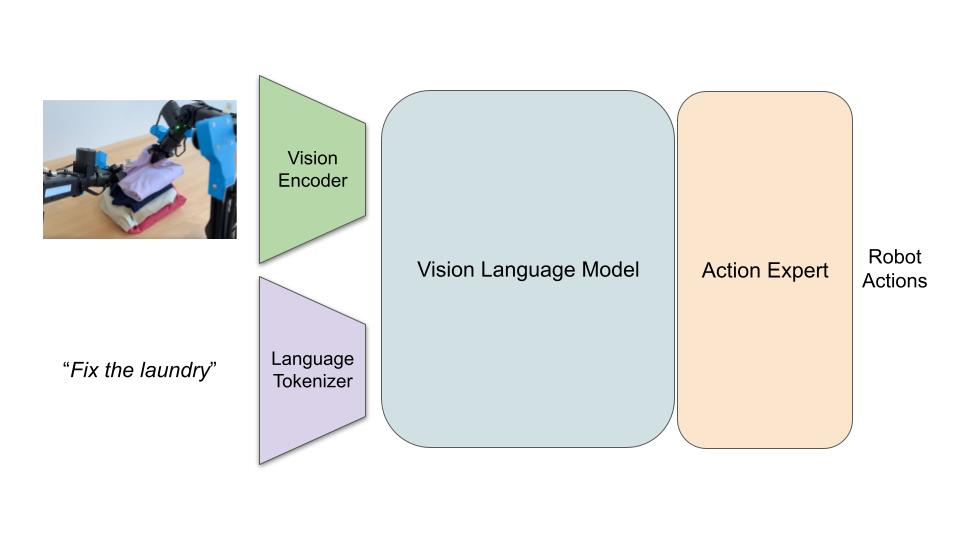
\includegraphics[width=0.45\textwidth]{images/vla.jpg}
    \caption{VLA abstraction}
    \label{fig:vla_abstraction}
    \vspace{-15pt}
    % https://docs.google.com/presentation/d/1F3-KIjQxwBtXfJAlc9_vwuBLSGuZqcXqZ7_GfxX5kYY/edit?usp=sharing
\end{wrapfigure}

Robotics foundational models, often referred to as Vision-Language-Action (VLA) models, are the policies 
emerging from this paradigm shift. This nomenclature reflects their modality: vision and language serve as inputs while 
actions serve as outputs (Figure \ref{fig:vla_abstraction}). Leveraging techniques such as Imitation Learning and 
Reinforcement Learning, these models have demonstrated remarkable capabilities in dexterous manipulation across multiple tasks, 
offering a degree of generalization over robot embodiments and environments. The key enablers of this progress are twofold: 
first, the usage of pretrained vision-language models (VLMs) trained on vast corpora of internet-scale data as an initial 
starting point, providing rich semantic understanding; and second, the collection of vast and varied robotics datasets 
which are used to train the VLA models to map visual and linguistic inputs to appropriate robotic actions.

\section{Goals and Objectives}
Due to the rapid pace of development in robotics foundation models, the field currently lacks established, comprehensive comparison benchmarks for complex interaction scenarios like deformable object manipulation (DOM).
This absence makes rigorous comparison between foundational models challenging, while simultaneously presenting an opportunity for standardization.
Although some models like $\pi_0$ \cite{pi_zero} have demonstrated capabilities in specific DOM tasks (Shirt/Towel/Laundry Folding), a standardized evaluation suite is still missing.
Such a suite is essential for equitable evaluation and deeper understanding of model capabilities across different manipulation scenarios.
As benchmarking is fundamentally a process of testing, therefore real-world evaluation is crucial for assessing true model performance. We will also employ simulation environments to scale our experiments and provide controlled testing conditions across a wider range of scenarios.

\subsection{Overall Goal}
The primary objective of this project is to develop DOM-Bench: a standardized benchmarking suite tailored for evaluating robotics foundation models on deformable object manipulation tasks. This will provide a coherent and equitable basis for comparing model capabilities and limitations.

This project aims to deliver:
\begin{itemize}
    \item DOM-Bench Suite: A set of deformable object manipulation tasks, environments, and metrics designed to evaluate robotics foundation models.
    \item Evaluation Protocol and Implementation: Specify the procedure for applying the benchmark suite to different models, e.g: specifications for data efficiency testing and implement the protocol on selected models.
    \item Summarization of the findings: write an accessible report of the results in the form of a workshop paper as a starting point for a potential publication.
\end{itemize}


\subsection{Specific Objectives}

\subsubsection{Literature Review} % Using subsubsection for better structure
The first task is to conduct a comprehensive review covering: existing robotics benchmarks, evaluation methodologies, and taxonomies, with a focus on deformable object manipulation and metrics used; Robotics foundation models (VLAs), detailing architectures, training data/recipes, and claimed capabilities relevant to manipulation.

\subsubsection{Benchmark Design (DOM-Bench)}
Following our review and drawing insights from existing benchmarks, for example in simulation SoftGym \cite{SoftGym} and GarmentLab \cite{GarmentLab}, we will propose DOM-Bench, a benchmark suite and evaluation protocol designed for evaluating robotics foundational models over Deformable Object Manipulation (DOM) tasks. The primary goal of DOM-Bench is to offer deeper insights into a model's capabilities, moving beyond simple task success rates.
To achieve this, DOM-Bench will employ a multi-tier task structure. Tasks are organized into tiers of increasing complexity, with each tier designed to evaluate distinct capabilities using specific, measurable metrics. (A detailed brainstorming of potential tasks can be found in Appendix~\ref{app:task_suite}).

In the following, we will discuss the specific components of DOM-Bench and our evaluation methodology, distinguishing between minimum requirements (core objectives essential for project success) and stretch goals (additional objectives to be pursued if time and resources permit).

\paragraph{\textbf{Primitive DOM manipulation} (Minimum Requirement)}
The first component of DOM-Bench will evaluate performance over a series of simple tasks (Appendix~\ref{app:task_suite_1}) designed to assess the core deformable object manipulation abilities of the models.

\begin{domexample}
For this component, we will select one task for each type of deformable object (rope 1D, fabric 2D and liquid 3D) from the DaXBench simulator - \{WhipRope, FoldTShirt, PourSoup\}. % This test will cover a single environment, and a single embodiment (since the DaXBench provides end effector control), therefore we will need to generate forward and inverse kinematics for coherence with the output of the models.
\end{domexample}

\paragraph{\textbf{Evaluating Data Efficiency} (Minimum Requirement)}
The second component of DOM-Bench will measure data efficiency by quantifying how model performance changes based on the amount of fine-tuning data provided. Specifically, we will record performance under different conditions: zero-shot (no fine-tuning examples), fine-tuned with 10 examples, fine-tuned with 30 examples.

\begin{domexample}
For this component, we will evaluate VLA models on a set of tasks: \{HangClothes, StoreInCloset, PourRice\}. HangClothes and StoreInCloset will be defined in GarmentLab \cite{GarmentLab}, while PourRice will be executed in the RPL lab (a real environment, where we can test different embodiments, e.g., SO-100 and Franka Panda from RPL).
To measure data efficiency comprehensively, we will aggregate performance across these variations. For a single VLA model, the total number of tests required would be calculated based on the variations per task: 1 (HangClothes) + 1 (StoreInCloset) + 2 (PourRice, one for each embodiment) = 4 variations. Each variation will be tested under 3 different data conditions \{ \text{0-shot, 10 demos, 30 demos} \} resulting in 12 tests.
\end{domexample}

This approach allows for measuring generalization across tasks, environments (simulation and real), and robot embodiments, similar to the methodology in \cite{TransferWelle}.

\paragraph{\textbf{Additional Benchmark Components} (Stretch Goals)}
Beyond our minimum requirements, we have identified several stretch goals to enhance DOM-Bench if time and resources permit:

\begin{itemize}
    \item \textbf{Further Tasks Expansion:} Include additional tasks for the core evaluation metrics.
    
    \item \textbf{Long-Horizon Planning Tasks:} Design specific long-horizon tasks (from Appendix~\ref{app:task_suite_3}) to quantitatively assess the effective context length a model can utilize for successful task completion with DOM.
    
    \item \textbf{Instruction Following Evaluation:} Develop tasks requiring precise instruction following to evaluate the model's ability to understand and execute complex language-conditioned tasks.
    
    \item \textbf{Vocabulary Generalization:} Create tasks testing the model's ability to generalize to new vocabulary, including novel objects and actions not seen during training.
    
    \item \textbf{Explainable AI Integration:} Incorporate methods (e.g., representational probing \cite{Probing-VLA}, attention analysis) to gain insights into the models' internal representations and decision-making processes during DOM tasks.
\end{itemize}

% \paragraph{Protocol Definition:} Define a precise experimental protocol specifying setup, initial state randomization, number of trials, permissible interventions (if any), and data logging requirements. Reference Appendix \ref{app:task_suite} for detailed task specifications.
\subsubsection{Evaluation \& Analysis}
The final phase of our project involves implementing the DOM-Bench evaluation protocol to comprehensively assess foundation model performance across both simulated and real-world settings.
We will initially focus on three publicly available models ($\pi_0$ \cite{pi_zero}, $\text{OpenVLA}$ \cite{OpenVLA}, and $\text{Gr00t}$ \cite{Gr00tN1}),
with potential expansion to include additional models ($\text{OpenVLA-OFT}$ \cite{OpenVLA-OFT} and $\text{Octo}$ \cite{Octo}) if time permits.
A central component of this evaluation will be deploying and adapting these models for real-world execution within the RPL laboratory environment,
which requires configuring the physical workspace with appropriate robotic hardware (e.g. a dual-camera system)
for model input and task execution, while establishing a reliable pipeline for collecting human demonstrations to serve as fine-tuning data.
Implementing the software to run the chosen models on the available RPL hardware will be a core technical challenge of the project as it may require adapting model inputs/outputs to match specific robot controllers and sensors.
Once this infrastructure is in place, we will gather a targeted dataset of demonstrations,
fine-tune the deployed models, and evaluate their performance on real-world DOM-Bench tasks according to our defined protocol.


\paragraph{Stretch Goals:}

Evaluation expansion can be achieved by adding additional models such as: $\text{OpenVLA-OFT}$ \cite{OpenVLA-OFT} and $\text{Octo}$ \cite{Octo}.


This comprehensive evaluation will establish baseline performance metrics for future research, highlight specific areas where current foundation models excel or require improvement.
